\documentclass{article}
\usepackage{graphics} 
\usepackage{hyperref}
\usepackage{fixltx2e}
\usepackage{amssymb}
\usepackage{tikz}

\author{Kevin Zollicoffer}
\title{Regression\\Lesson 2b}
\date{10/21/2013}

% no indents
\setlength\parindent{0pt}

\usepackage{Sweave}
\begin{document}
\maketitle
%\tableofcontents
\Sconcordance{concordance:Assignment2b.tex:Assignment2b.Rnw:%
1 14 1 1 0 56 1 1 2 4 0 1 2 1 1 1 2 1 0 1 1 29 0 1 2 5 1 1 2 1 0 1 1 22 %
0 1 2 3 1 6 0 1 2 2 1 1 2 1 0 2 1 26 0 1 2 28 1 1 2 5 0 2 2 1 0 2 1 4 0 %
2 2 5 0 2 2 5 0 2 2 5 0 2 2 5 0 2 2 5 0 2 2 1 0 1 1 4 0 1 3 5 0 1 2 6 1 %
1 2 1 0 1 1 7 0 1 2 1 1 1 2 8 0 1 2 1 1}


\section*{Introduction}
Regression assignment 2b using R
\\
\\
The complete source for this assigment is available on Github:
\\
\\
\url{https://github.com/zollie/PASS-Regression-Assignment2b}

\section*{Problem 3.5}
\subsection*{a}
$E(Att) = 28.721+1.350Pop-.972Teams-.238Temp$
\\\\
or
\\\\
$\hat{Att} = 28.721+1.350Pop-.972Teams-.238Temp$
\\\\
\subsection*{b}
Global usefulness test
\\\\
$H_0=b_0=b_1=b_2=0$
\\\\
$H_a=b_0\neq0 \lor b_1\neq0 \lor b_2\neq0$
\\\\
significance level is 5\% $(1-.95 = .05)$ for upper tail test
\\\\
$R^2=.914$
$k=3$
$n=12$
\\\\
F-statistic$={R^2/k \over (1-R^2)/(n-k-1)}={.914/3 \over (1-.914)/(12-3-1)}={.3046687 \over .01075}=28.27907$
\\\\
$28.279 > 4.07$ therefore we reject $H_0$

\subsection*{c}
$H_0=b_1=0$
\\
$H_a=b_1<0$
\\
p-value$=.037/2=.0185$

.0185 < .05 therefore reject $H_0$
\\\\
This suggestes the model predicts a non-zero drop in attendence for each additional male major professional sports team to an MLS city. 

\subsection*{d}
The coefficient for Teams is -0.972, therefore for every additional male professional major sport team, all other things constant, the model predicts a decline of 972,000 attedees for that cities MLS franchise. 

\subsection*{e}
Presumably, home attendance for a sports franchise is the major source of revenue for a team. These attendees pay a ticket fee to attend the game. Knowing the fee, a potential team, or league can determine the break even point for attendence given the potential location of the team. A model such as this gives a data driven, objective, decision making tool that can help determine whether a potential location is viable for an MLS franchise.  

\section*{Problem 3.6}
\begin{Schunk}
\begin{Sinput}
> smsa <- read.csv("~/R/PASS/Regression/Assignment2b/smsa.csv")
\end{Sinput}
\end{Schunk}

\subsection*{a}
\begin{Schunk}
\begin{Sinput}
> model <- lm(Mort ~ Edu+Nwt+Jant+Rain+Nox+Hum+Inc, data=smsa)
> summary(model)
\end{Sinput}
\begin{Soutput}
Call:
lm(formula = Mort ~ Edu + Nwt + Jant + Rain + Nox + Hum + Inc, 
    data = smsa)

Residuals:
    Min      1Q  Median      3Q     Max 
-84.380 -22.118   2.907  23.154  77.369 

Coefficients:
             Estimate Std. Error t value Pr(>|t|)    
(Intercept) 1006.2441    95.0827  10.583 3.84e-14 ***
Edu          -15.3459     7.2515  -2.116  0.03954 *  
Nwt            4.2140     0.6850   6.152 1.47e-07 ***
Jant          -2.1500     0.6593  -3.261  0.00204 ** 
Rain           1.6238     0.5643   2.878  0.00596 ** 
Nox           18.5481     5.5065   3.368  0.00150 ** 
Hum            0.5371     0.9024   0.595  0.55451    
Inc           -0.3453     1.3038  -0.265  0.79227    
---
Signif. codes:  0 ‘***’ 0.001 ‘**’ 0.01 ‘*’ 0.05 ‘.’ 0.1 ‘ ’ 1

Residual standard error: 35.48 on 48 degrees of freedom
Multiple R-squared:  0.7137,	Adjusted R-squared:  0.6719 
F-statistic: 17.09 on 7 and 48 DF,  p-value: 4.183e-11
\end{Soutput}
\end{Schunk}
$\hat{Y} = 1006.2441-15.3459Edu+4.2140Nwt-2.15Jant+1.6238Rain+18.5481Nox+.5371Hum-.3453Inc$

\subsection*{b}
$H_0=Hum=Inc=0$
\\
$H_a=Hum\neq0 \lor Inc\neq0$
\begin{Schunk}
\begin{Sinput}
> model0 <- lm(Mort ~ Hum+Inc, data=smsa)
> summary(model0)
\end{Sinput}
\begin{Soutput}
Call:
lm(formula = Mort ~ Hum + Inc, data = smsa)

Residuals:
     Min       1Q   Median       3Q      Max 
-118.372  -39.302    1.274   43.194  170.185 

Coefficients:
             Estimate Std. Error t value Pr(>|t|)    
(Intercept) 1118.9420    98.7427  11.332 8.88e-16 ***
Hum           -0.8753     1.4979  -0.584   0.5615    
Inc           -3.7213     1.8264  -2.038   0.0466 *  
---
Signif. codes:  0 ‘***’ 0.001 ‘**’ 0.01 ‘*’ 0.05 ‘.’ 0.1 ‘ ’ 1

Residual standard error: 60.35 on 53 degrees of freedom
Multiple R-squared:  0.08512,	Adjusted R-squared:  0.0506 
F-statistic: 2.466 on 2 and 53 DF,  p-value: 0.09466
\end{Soutput}
\begin{Sinput}
> k <- 2
> n <- nrow(smsa)
> df2 <- n-k-1
> qf(0.05, k, df2, lower.tail=F)
\end{Sinput}
\begin{Soutput}
[1] 3.171626
\end{Soutput}
\end{Schunk}
2.466 < 3.17 therefore we do not reject $H_0$. The coefficients for Hum and Inc may be statistically 0.

\subsection*{c}
\begin{Schunk}
\begin{Sinput}
> options(scipen=999) # disable scientific notation
> modelr <- lm(Mort ~ Edu+Nwt+Jant+Rain+Nox, data=smsa)
> summary(modelr)
\end{Sinput}
\begin{Soutput}
Call:
lm(formula = Mort ~ Edu + Nwt + Jant + Rain + Nox, data = smsa)

Residuals:
    Min      1Q  Median      3Q     Max 
-86.139 -24.728   4.088  21.200  79.659 

Coefficients:
             Estimate Std. Error t value             Pr(>|t|)    
(Intercept) 1028.2323    84.9148  12.109 < 0.0000000000000002 ***
Edu          -15.5887     6.4460  -2.418              0.01927 *  
Nwt            4.1807     0.6600   6.334          0.000000066 ***
Jant          -2.1313     0.6369  -3.347              0.00156 ** 
Rain           1.6331     0.5551   2.942              0.00493 ** 
Nox           18.4132     5.2926   3.479              0.00105 ** 
---
Signif. codes:  0 ‘***’ 0.001 ‘**’ 0.01 ‘*’ 0.05 ‘.’ 0.1 ‘ ’ 1

Residual standard error: 34.91 on 50 degrees of freedom
Multiple R-squared:  0.7111,	Adjusted R-squared:  0.6822 
F-statistic: 24.62 on 5 and 50 DF,  p-value: 0.000000000002044
\end{Soutput}
\end{Schunk}
\subsubsection*{Edu}
$H_0=Edu=0$
$H_a=Edu \neq 0$
\\
p-value of 0.0000000000000002 < 0.025 therefore reject $H_0$
\subsubsection*{Nwt}
$H_0=Nwt=0$
$H_a=Nwt \neq 0$
\\
p-value of 0.01927 < 0.025 therefore reject $H_0$
\subsubsection*{Jant}
$H_0=Jant=0$
$H_a=Jant \neq 0$
\\
p-value of 0.000000066 < 0.025 therefore reject $H_0$
\subsubsection*{Rain}
$H_0=Rain=0$
$H_a=Rain \neq 0$
\\
p-value of 0.00493 < 0.025 therefore reject $H_0$
\subsubsection*{Nox}
$H_0=Nox=0$
$H_a=Nox \neq 0$
\\
p-value of 0.00493 < 0.025 therefore reject $H_0$

\subsection*{d}
Random error assumptions

\begin{Schunk}
\begin{Sinput}
> scatter.smooth(fitted(modelr))
\end{Sinput}
\end{Schunk}
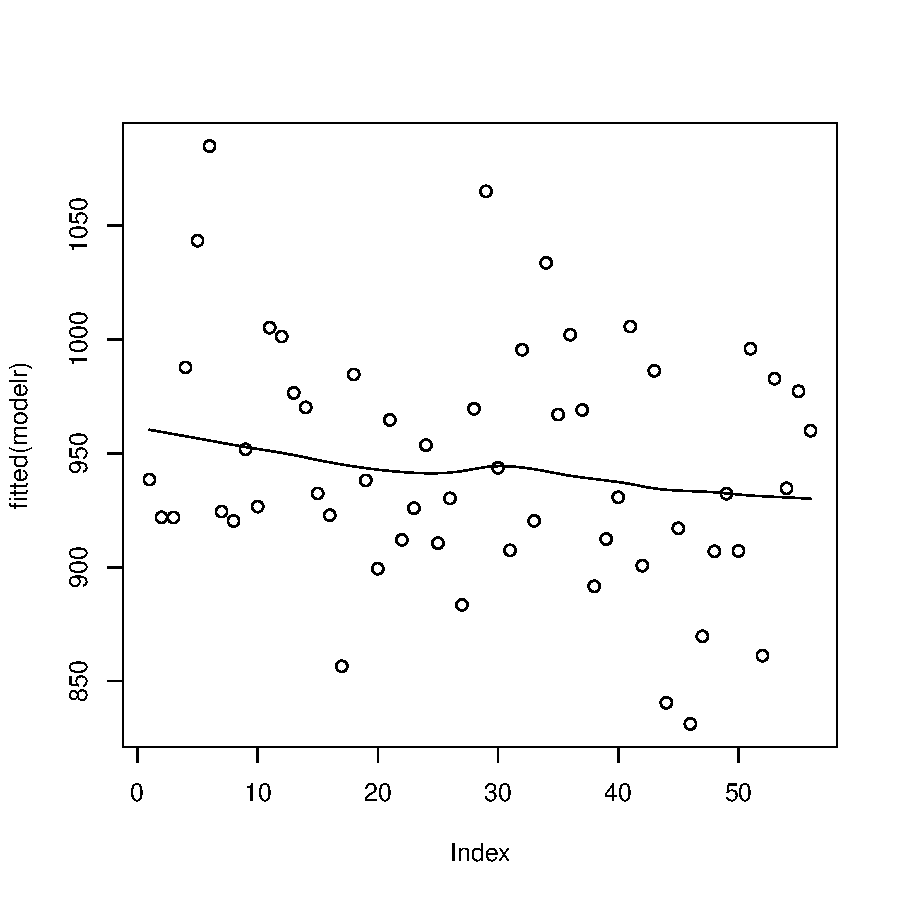
\includegraphics{Assignment2b-005}

\begin{Schunk}
\begin{Sinput}
> res <- residuals(modelr)
> fitted <- predict(modelr)
> plot(smsa$Edu, res)
\end{Sinput}
\end{Schunk}
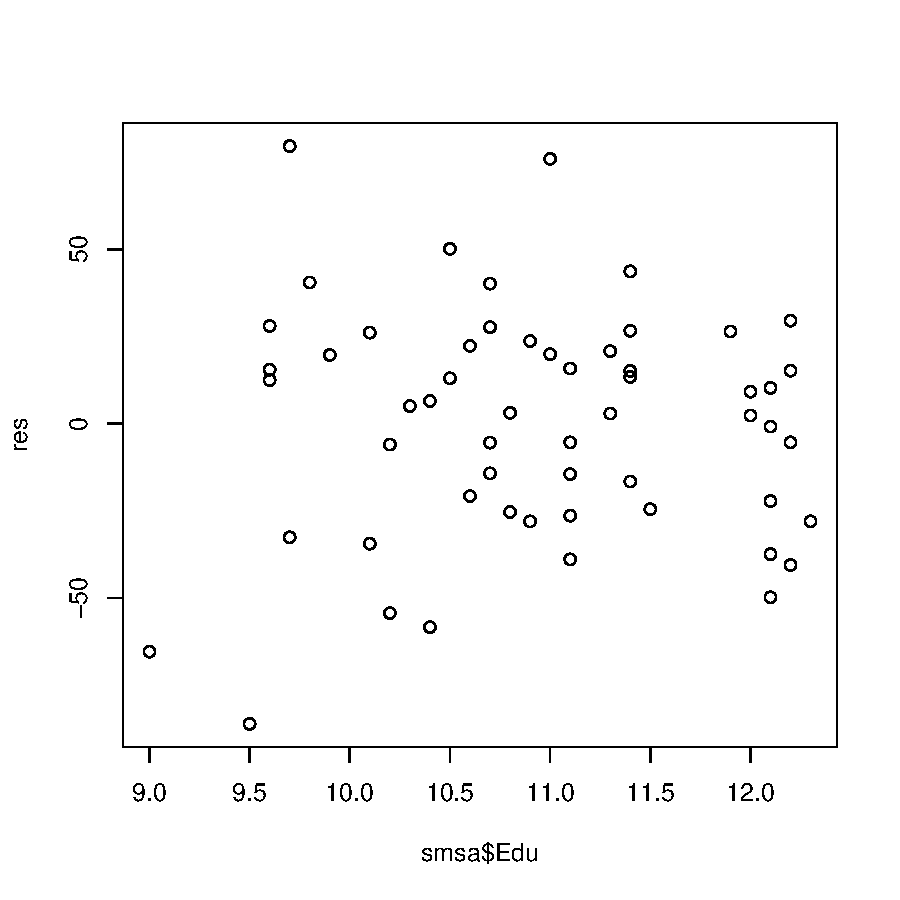
\includegraphics{Assignment2b-006}

\begin{Schunk}
\begin{Sinput}
> plot(smsa$Nwt, res)
\end{Sinput}
\end{Schunk}
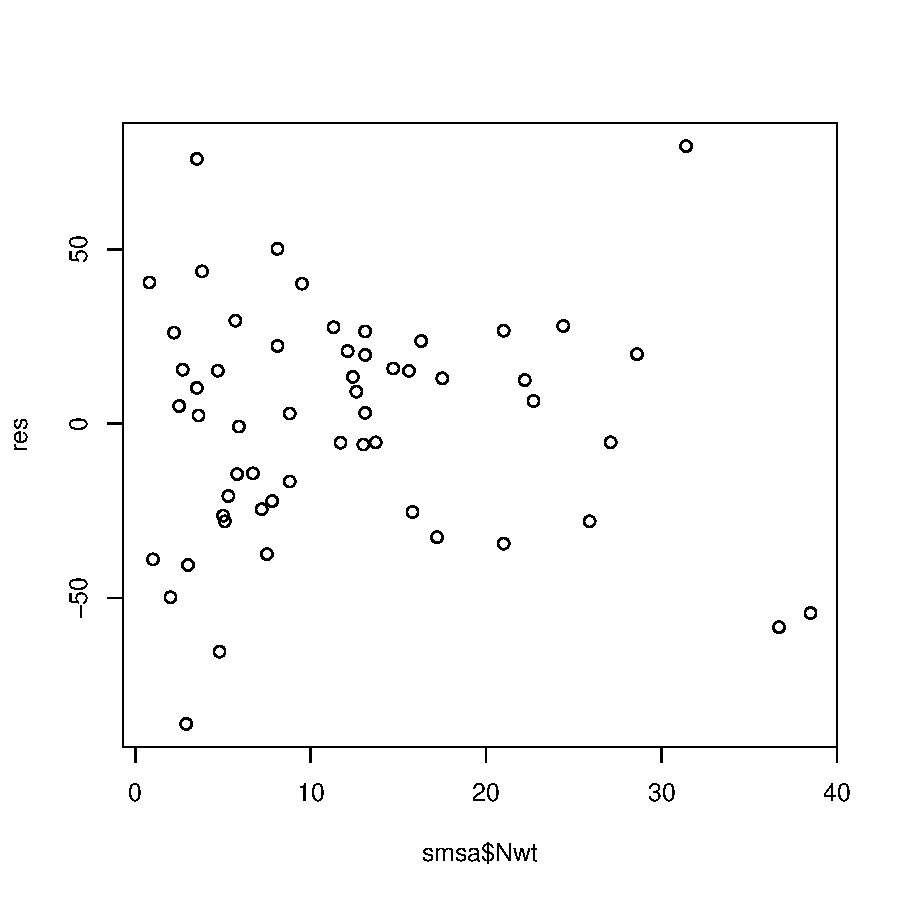
\includegraphics{Assignment2b-007}

\begin{Schunk}
\begin{Sinput}
> plot(smsa$Jant, res)
\end{Sinput}
\end{Schunk}
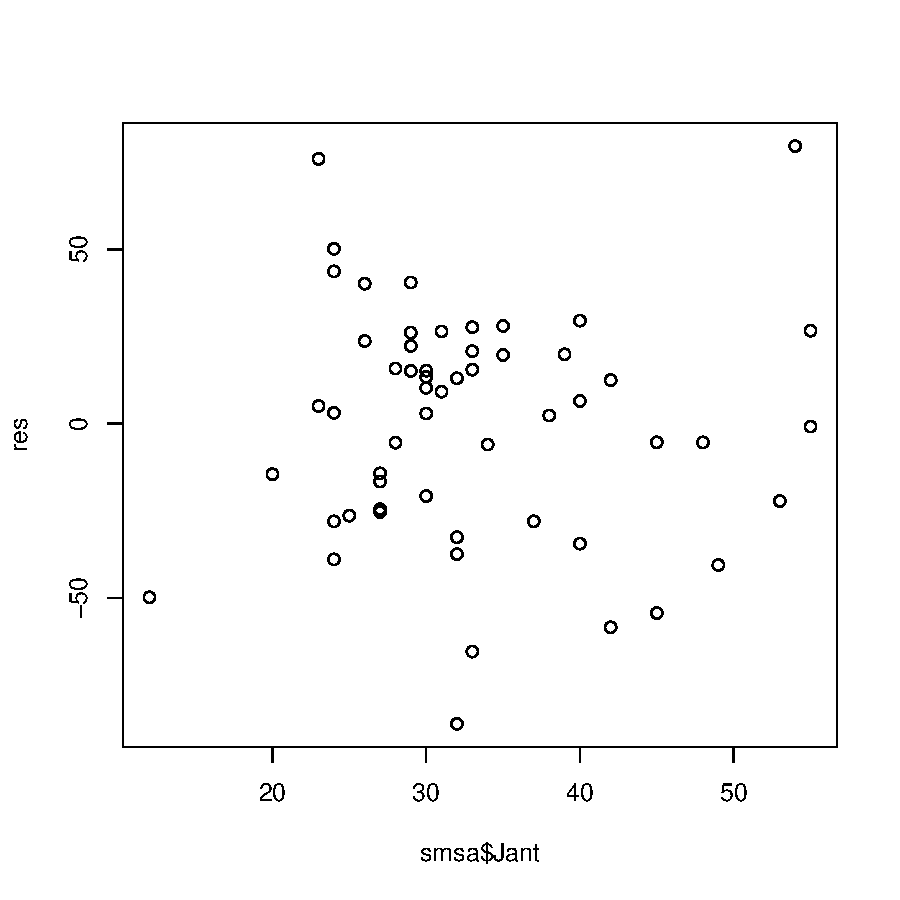
\includegraphics{Assignment2b-008}

\begin{Schunk}
\begin{Sinput}
> plot(smsa$Rain, res)
\end{Sinput}
\end{Schunk}
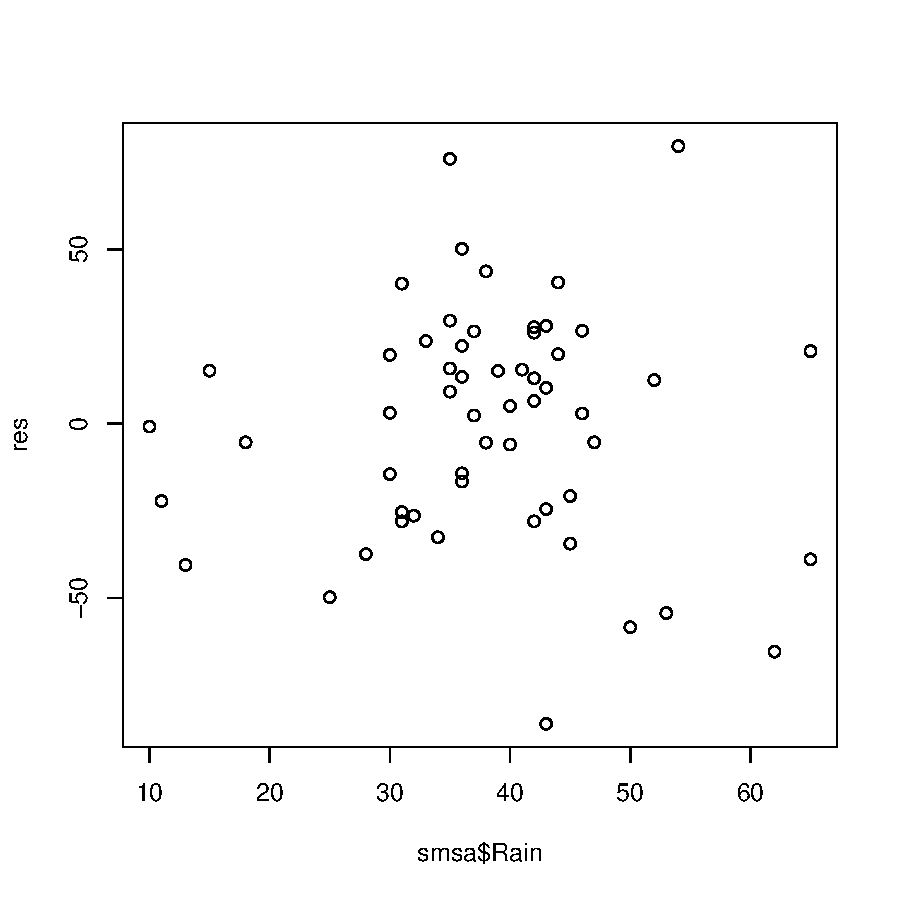
\includegraphics{Assignment2b-009}

\begin{Schunk}
\begin{Sinput}
> plot(smsa$Nox, res)
\end{Sinput}
\end{Schunk}
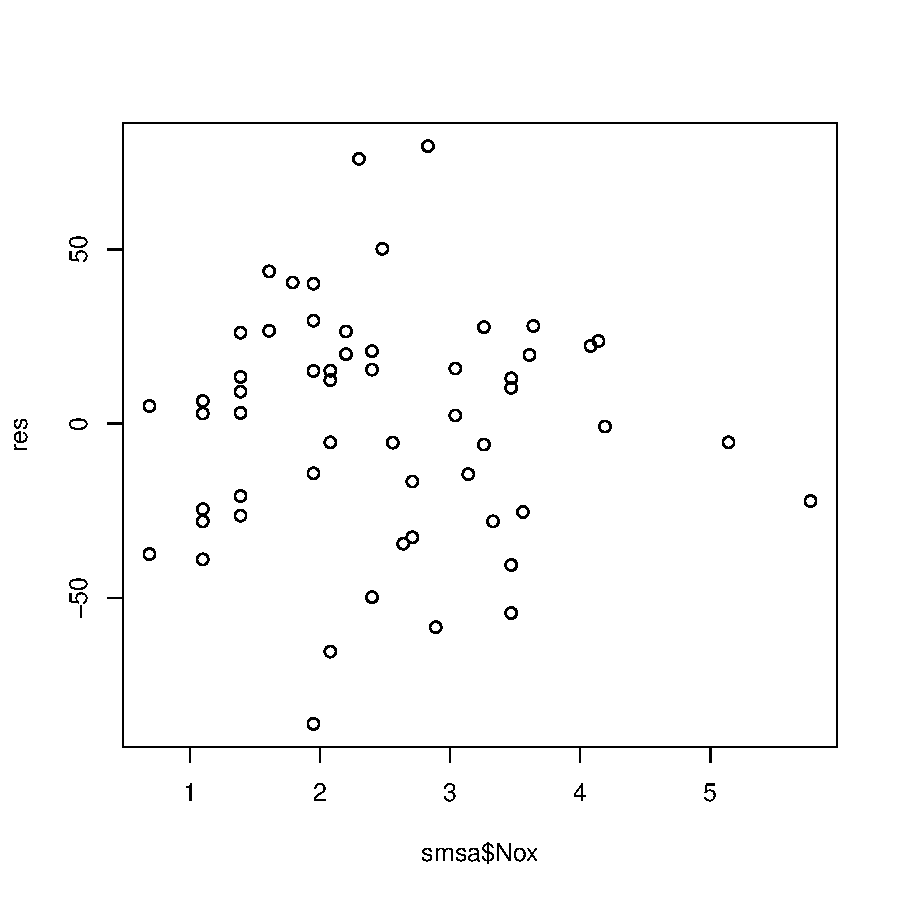
\includegraphics{Assignment2b-010}

\begin{Schunk}
\begin{Sinput}
> plot(fitted, res)
\end{Sinput}
\end{Schunk}
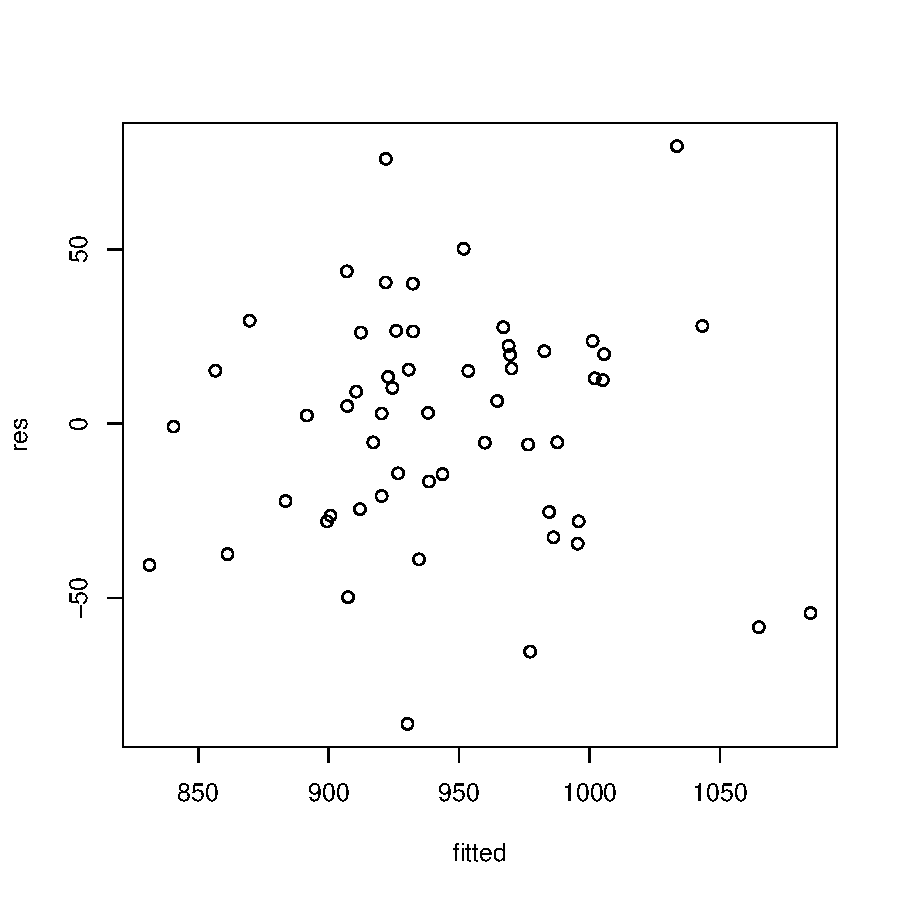
\includegraphics{Assignment2b-011}

\begin{Schunk}
\begin{Sinput}
> qqnorm(res)
> qqline(res)
\end{Sinput}
\end{Schunk}
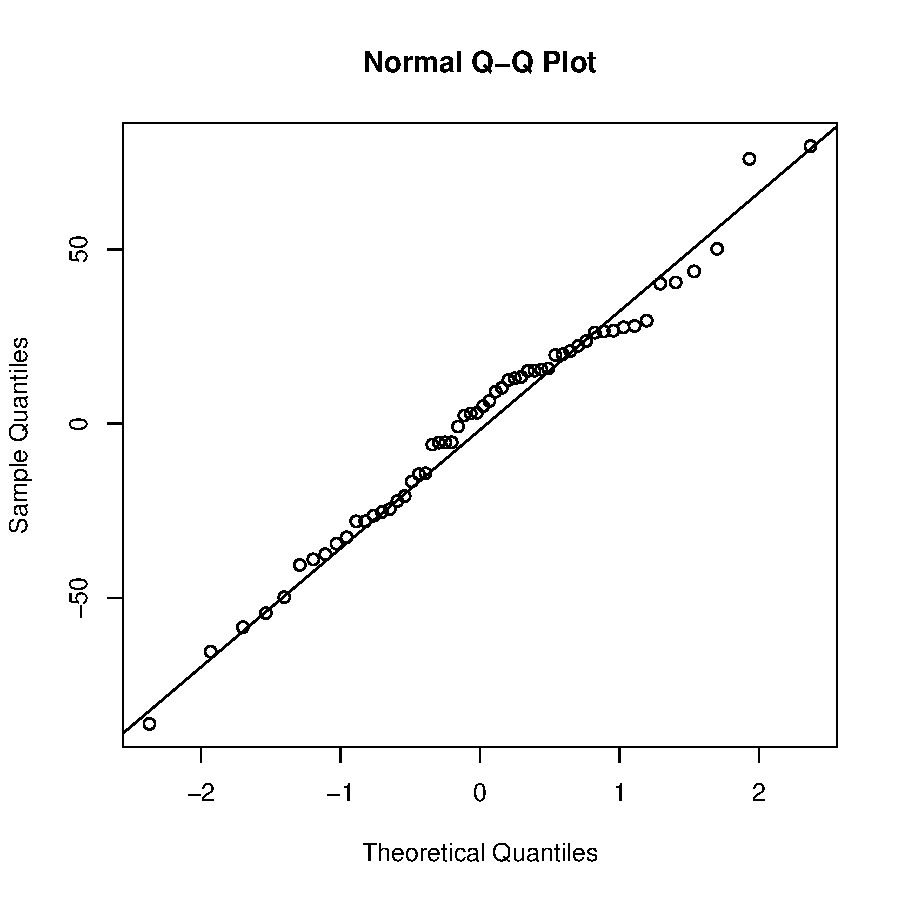
\includegraphics{Assignment2b-012}
\begin{Schunk}
\begin{Sinput}
> hist(res, freq=T)
\end{Sinput}
\end{Schunk}
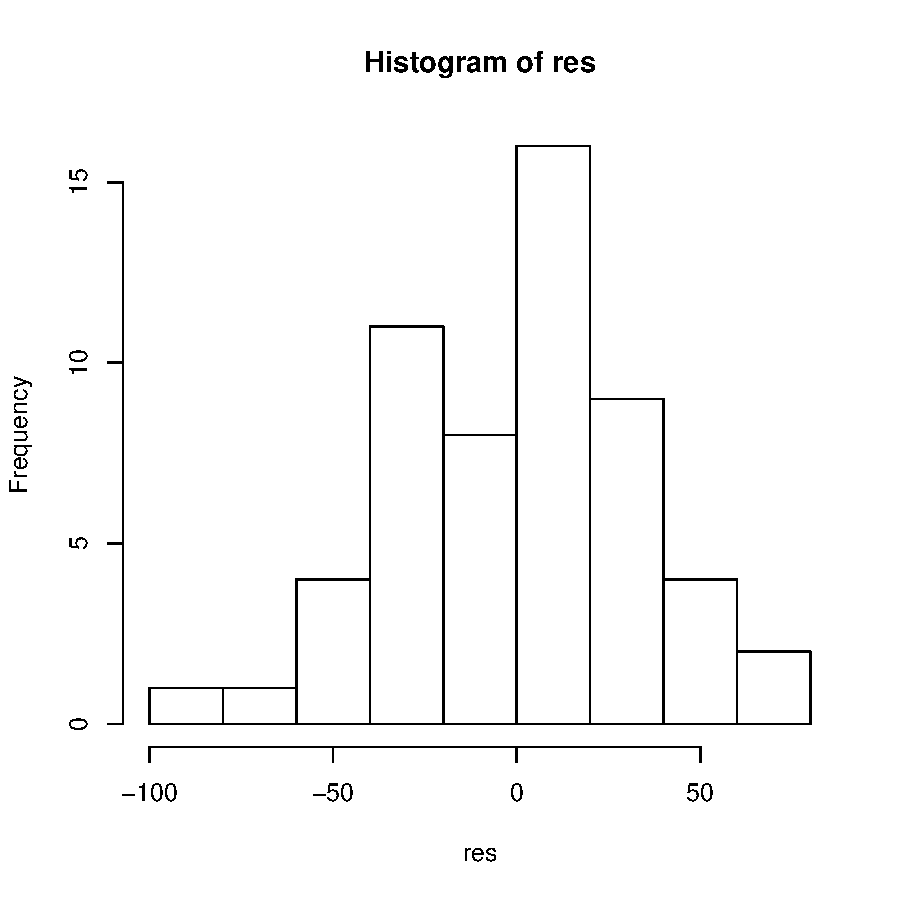
\includegraphics{Assignment2b-013}

\subsection*{e}
$\hat{Y}=1028.2323-15.5887Edu+4.1807Nwt-2.1313Jant+1.6331Rain+18.4132Nox$
\\\\
The signs of the estimated regression parameters make sense in this context in a few ways. Life expectancy increeases with the level of education (the rate of mortality declines), the rate of mortality incresases as the amount of NO gas in the atmosphere increases. Mortality increases with amount of rain as well, perhaps due to accidents.  

\subsection*{f}
\begin{Schunk}
\begin{Sinput}
> nd <- data.frame(Edu=10,Nwt=15,Jant=35,Rain=40,Nox=2)
> predict(modelr, newdata=nd, interval="confidence")
\end{Sinput}
\begin{Soutput}
       fit      lwr      upr
1 962.6092 946.2731 978.9454
\end{Soutput}
\end{Schunk}

\subsection*{g}
\begin{Schunk}
\begin{Sinput}
> predict(modelr, newdata=nd, interval="prediction")
\end{Sinput}
\begin{Soutput}
       fit      lwr      upr
1 962.6092 890.6053 1034.613
\end{Soutput}
\end{Schunk}

\end{document}
